\documentclass{beamer}
\usepackage{graphics}
\usepackage{epsfig}
\usepackage{multicol}
\usepackage{pifont}
\setbeamertemplate{navigation symbols}{}
\newcommand{\RR}{\ensuremath{\mathbb{R}}}
\newcommand{\NN}{\ensuremath{\mathbb{N}}}
\newcommand{\QQ}{\ensuremath{\mathbb{Q}}}
\newcommand{\CC}{\ensuremath{\mathbb{C}}}
\newcommand{\ZZ}{\ensuremath{\mathbb{Z}}}
\newcommand{\TT}{\ensuremath{\mathbb{T}}}
\newcommand{\HH}{\ensuremath{\mathbb{H}}}
\DeclareMathOperator{\Min}{Min}
\DeclareMathOperator{\mint}{min}
\DeclareMathOperator{\vertt}{vert}
\DeclareMathOperator{\conv}{conv}
\DeclareMathOperator{\rank}{rank}
\DeclareMathOperator{\tdiv}{div}

\begin{document}
\title{New developments in the WaveWatch III model}
\author{
\begin{center}
\textcolor{red}{\large Mathieu Dutour Sikiri\'c}\\[2mm]
\textcolor{red}{Rudjer Bo\u skovi\'c Institute, Croatia}\\[2mm]
\textcolor{red}{and Universit\"at Rostock}
\end{center}
}

\date{\today} 
\frame{\titlepage} 








\frame{
\begin{center}
\begin{tabular*}{7cm}{c}
\\[-0.5cm]
{\Huge \textcolor{blue}{I. }\textcolor{red}{Wave models}}
\end{tabular*}
\end{center}
}

\frame{
  \frametitle{Stochastic wave modelling}

\begin{itemize}
\item Oceanic models are using grids (structured or unstructured) of size $1km\leq d\leq 10km$ to simulate the ocean
\item But oceanic waves have a typical wavelength $2m$ $\leq$ $L$ $\leq$ $100m$. So, we cannot resolve waves in the ocean.
\item But if one uses phase averaged models and uses stochastic assumptions
then it is possible to model waves by a spectral wave action density
$N({\bf x},{\bf k})$
\item This density satisfies a Wave Action Equation (\textcolor{red}{WAE}) which represents advection, refraction, frequency shifting and source terms:
\begin{equation*}
\frac{\partial N}{\partial t} + \nabla_x(({\bf c}_g+{\bf u}_A)N) + \nabla_k(\dot{k} N) 
 + \nabla_{\theta}(\dot{\theta} N) = S_{tot}
\end{equation*}
with
\begin{equation*}
S_{tot} = S_{in} + S_{nl3} + S_{nl4} + S_{bot} + S_{ds} + S_{break} + S_{bf}
\end{equation*}
\end{itemize}
}





\frame{
\begin{center}
\begin{tabular*}{7cm}{c}
\\[-0.5cm]
{\Huge \textcolor{blue}{II. }\textcolor{red}{The WaveWatch III}}\\[4mm]
{\Huge \textcolor{red}{model}}
\end{tabular*}
\end{center}
}


\frame{
  \frametitle{The WWM model}
It is a simpler model authored by Aron Roland and which shares many common features with WaveWatch III.
\begin{itemize}
\item It is comparable to WaveWatch III, SWAN, WAM or SWAVE.
\item The Wind Wave Model (WWM) is a unstructured grid spectral wave model.
\item It incorporates most existing source term formulation for wind input and dissipation (Cycle III, Cycle IV, Ardhuin, Makin, ...)
\item It has been coupled to SELFE, SHYFEM, TIMOR and ROMS.
\item It uses Residual Distribution schemes for the horizontal advection.
\item It integrates the WAE by using the Operator Splitting Method in explicit or implicit mode.
\end{itemize}
}



\begin{frame}[fragile]
  \frametitle{Features of WaveWatch III}

\begin{itemize}
\item It supports both Structured grids and Unstructured grids.
\item It has a nested grid approach, i.e. we can have a global model running all over the globe and subgrids (Structured or not) running locally.
\item It has parametrizations of source terms for wavegrowth and decay due to wind, nonlinear resonant interactions, dissipation (whitecapping), bottom friction, surf breaking and scattering due to wave-bottom interactions.
\item Also included are triad (shallow water) and quadruplets nonlinear interactions between waves.
\item The model has support for water level, current, tidal forcing, wet and dry, ice coverage used from forcing data.
\item It has a coupled module with MARS3D model.
\item As a consequence it is used in operational runs by many institutes (NOAA, IFREMER, etc.)
\end{itemize}
\end{frame}






\begin{frame}[fragile]
  \frametitle{Options choices in WW3}
\begin{itemize}
\item Like in {\tt ROMS}, WW3 is based on a choice of options that are first compiled.
\item Those options are stored in a  {\tt bin/switch} file that stores them
\item In {\tt ROMS} the {\tt cpp} preprocessor is used and this uses
\begin{verbatim}
#ifdef NOLA
 ..
#else
# ifndef XXX
# endif
#endif
\end{verbatim}
\item But in contrast to {\tt ROMS} the options are used in the code as
\begin{verbatim}
!/PR1     
\end{verbatim}
\item This gives less flexibility because {\tt CPP} is a true language while those options are not.

\end{itemize}
\end{frame}




\begin{frame}[fragile]
  \frametitle{Compilation in WW3}
\begin{itemize}
\item The WW3 has a very intricate compilation system based on bash scripts:
\begin{verbatim}
w3_clean
w3_new
w3_make
\end{verbatim}
\item We replaced it by a new compilation, more robust, system based on a single makefile. It can so compile on multiprocessors via
\begin{verbatim}
make -j 4
\end{verbatim}
\item In any case, even in coupled systems, we need to have one single makefile and avoid recursive makefiles.
\item In all cases dependencies between files are computed by script (bash or perl) and inserted into the makefile.
\end{itemize}
\end{frame}


\frame{
  \frametitle{Parallelization in WW3}
\begin{itemize}
\item Parallelization in WW3 can be done either via OpenMP or via MPI.
\item If one uses MPI, then there are three arrays
\begin{enumerate}
\item Arrays {\tt (NY, NX)} for the geographic information (NY=1 for unstructured)
\item Array {\tt (1:NSEA)} for the sea points
\item Array {\tt (1:NSEAL)} for the local 
\end{enumerate}
\item The classical parallelization system used in WW3 uses:
\begin{enumerate}
\item source term integration, refraction and frequency shifting are integrated on {\tt (1:NSEAL)} (so with geographic parallelization)
\item The advection is integrated on {\tt (1:NSEA)} (so with frequency parallelization)
\end{enumerate}
\item This requires a lot of exchange when one passes from one mode to the other.
\item We therefore implemented a scheme that used geographic parallelization

\end{itemize}
}


\frame{
\begin{center}
\begin{tabular*}{7cm}{c}
\\[-0.5cm]
{\Huge \textcolor{blue}{II. }\textcolor{red}{Numerical solutions}}\\[4mm]
{\Huge \textcolor{red}{methods}}
\end{tabular*}
\end{center}
}




\frame{
  \frametitle{The CFL criterion}
\begin{itemize}
\item If the discretization has characteristic length $l$ and the physical speed is $c$ then we have the condition
\begin{equation*}
\frac{ c \Delta t}{l} \leq 1
\end{equation*}
\item For the integration of the frequency and directional equations we can subdivide the integration time step if necessary because everything is decoupled.
\item This is not possible for the geographical advection:
\begin{itemize}
\item The dependency in direction/frequency is small or negligible
\item The problem is that the group speed is $\sqrt{g h}$ and so the CFL number varies with the depth and the resolution.
\end{itemize}
\item So, we will present an implicit scheme for integrating $N_1$, i.e. in order to avoid the CFL limitation for advection.
\item Remark: the advection scheme used in implicit mode in WWM is the residual distribution scheme PSI.
\end{itemize}
}




\frame{
  \frametitle{Operator Splitting Method}
\begin{itemize}
\item A standard technique for integrating partial differential equations is the operator splitting method.
\item Over the interval $[t_0, t_1]$ we successively solve the equations
\begin{equation*}
\left\lbrace\begin{array}{rcl}
\frac{\partial N_1}{\partial t} + \nabla_{\theta}(\dot{\theta} N_1) = 0  &\mbox{~with~}& N_1(t_0)=N(t_0)\\ 
\frac{\partial N_2}{\partial t} + \nabla_k(\dot{k} N_2) = 0  &\mbox{~with~}& N_2(t_0)=N_1(t_1)\\ 
\frac{\partial N_3}{\partial t} + \nabla_x(({\bf c}_g+{\bf u}_A)N_3) = 0 &\mbox{~with~}& N_3(t_0) = N_2(t_1)\\
\frac{\partial N_4}{\partial t} = S(t) &\mbox{~with~}& N_4(t_0) = N_3(t_1)\\
\end{array}\right.
\end{equation*}
and we set $N(t_1)=N_4(t_1)$.
\item No matter what the order of the successive integration schemes is the final order will be $1$.
\item It it is possible to have higher order by more complex integration procedures (Strang splitting, iterative splitting, etc.)
\end{itemize}
}

\frame{
  \frametitle{Implicit method}
\begin{itemize}
\item In order to work around the CFL condition, one standard method is to use implicit methods i.e. to solve:
\begin{equation*}
\frac{dx}{dt} = f(x)
\end{equation*}
by writing $x^{n+1} = x^n + \delta t \times f\left(x^{n+1}\right)$.
\item This can be done for geographic advection.
\item But can also include refraction, frequency shifting.
\item It is also possible to integrate the source terms implicitly by Patankar linearization rule.
\item The problem is then to solve the corresponding linear systems
\begin{itemize}
\item Our first step is to introduce a geographical parallelization that minimize the interaction between blocks with PARMETIS.
\item Our method is then to use the PETSC library for solving the correspondings linear systems using iterative methods.
\end{itemize}
\item An additional benefit of integrating the WAE globally is to remove the splitting errors.
\end{itemize}
}










\frame{
\begin{center}
\begin{tabular*}{7cm}{c}
\\[-0.5cm]
{\Huge \textcolor{blue}{II. }\textcolor{red}{Wave setup}}
\end{tabular*}
\end{center}
}


\frame{
  \frametitle{Effect of waves on current}
\begin{itemize}
\item According to the classical Longuet-Higgins theory, if one takes the shallow water equations, in order to model the effect of the waves one needs to introduce the following force ${\bf F}_{wave} = (F_{wave,x}, F_{wave,y})$:
\begin{equation*}
\left\{\begin{array}{rcl}
F_{wave,x} &=& -\frac{\partial \overline{S}_{xx}}{\partial x} -\frac{\partial \overline{S}_{xy}}{\partial y}\\
F_{wave,y} &=& -\frac{\partial \overline{S}_{xy}}{\partial x} -\frac{\partial \overline{S}_{yy}}{\partial y}
\end{array}\right.
\end{equation*}
\item The potentials $\overline{S}_{\alpha\beta}$ are obtained by integration over the wave spectrum.
\item If one has a static solution then one gets the following equation:
\begin{equation*}
{\bf F}_{wave} + d {\bf grad} z = 0
\end{equation*}
\item Instead of using coupling, one may wish to solve the static equation.
\end{itemize}
}

\frame{
  \frametitle{The equation system}
\begin{itemize}
\item The exact equation is overdetermined as is natural due to our static assumption. In
\begin{itemize}
\item Dingemans, M.W., 1997.
Water wave propagation over uneven bottoms. Part 1 - linear wave propagation.
Advanced Series on Ocean Engineering, 13, World Scientific, 471 p.
\end{itemize}
It is asserted that the wav setup is mainly due to the rotation-free part of the force field.
\item Therefore by taking the divergence and adding a boundary condition we get the following system:
\begin{equation*}
\left\{\begin{array}{rcl}
\tdiv\left( {\bf F}_{wave} + d {\bf grad} z\right) &=& 0\mbox{~for~}x\in \Omega\\
{\bf n}\cdot \left( {\bf F}_{wave} + d {\bf grad} z\right) &=& 0\mbox{~for~}x\in \partial \Omega
\end{array}\right.
\end{equation*}
\item The system can be solved by Finite Elements and using preconditioned conjugate gradients.

\end{itemize}
}




\frame{
\begin{center}
\begin{tabular*}{7cm}{c}
\\[-0.5cm]
{\Huge \textcolor{blue}{II. }\textcolor{red}{Model coupling}}\\[4mm]
{\Huge \textcolor{red}{with PGMCL}}
\end{tabular*}
\end{center}
}

\frame{
  \frametitle{Model coupling library, {\tt PGMCL} }
\begin{itemize}
\item The exchange between models requires the sending of data between them.
\item A priori the grids are different, the model nature may be different (Structure/Unstructured grids) and so interpolation is needed between the models.
\item There are several existing libraries {\tt MCT}, {\tt OASIS}, {\tt PALM}, etc but when considering them, they appear all relatively complicated.
\item We considered {\tt MCT} and it appeared to be impossible to achieve the goals that we wanted (optimal exchanges, interpolation, performance, etc.).
\item Henceforth, we designed our own library {\tt PGMCL} (Parallel Geophysical Model Coupling Library) for coupling models.
\item After declarations, the commands become as simple as
\begin{center}
{\tt CALL MPI\_INTERP\_SEND(TheArr\_WAVtoOCN, Hwave)}\\
{\tt CALL MPI\_INTERP\_RECV(TheArr\_WAVtoOCN, Hwave)}
\end{center}

\end{itemize}
}


\frame{
  \frametitle{Coupling of {\tt WAM} and {\tt COSMO}}
\begin{itemize}
\item The {\tt WAM} model, originally the first $3^{rd}$ generation wave model, is a wave model used by many institutions  in the world.
\item The {\tt COSMO} model is based on the Lokall modell of DWD.
\item Both are finite difference models that are coupled via {\tt PGMCL}
\begin{itemize}
\item The atmospheric model provides the wind and air density to wave model.
\item The wave model provides the Charnock coefficient to the atmospheric model.
\end{itemize}
\item Results on the Mediterranean indicate a slight decrease of wind magnitude and an overall improvements in wave and wind statistics when comparing with altimeter and stations.

\end{itemize}
Work done in collaboration with P. Janssen/J. Bidlot (ECMWF), L. Cavaleri (ISMAR), L. Torrisi (CNMCA, Italian Nat. Met. Center) and A. Roland (TU Darmstadt)
}



\frame{
\begin{center}
\begin{tabular*}{7cm}{c}
\\[-0.5cm]
{\Huge \textcolor{blue}{II. }\textcolor{red}{Examples}}
\end{tabular*}
\end{center}
}



\frame{
  \frametitle{WaveWatch III coarse/fine grids}

\begin{itemize}
\item The WaveWatch III model uses the SCRIP library for computing interpolation coefficients. It gives conservative coefficients and the results are stable if one iterates coarse $\rightarrow$ fine $\rightarrow$ coarse.
\item Below, one can see a coarse FD grid with an embedded FE grid. The results of the FE grid is then interpolated 
\end{itemize}
\begin{center}
\begin{minipage}{3.9cm}
\centering
\resizebox{3.9cm}{!}{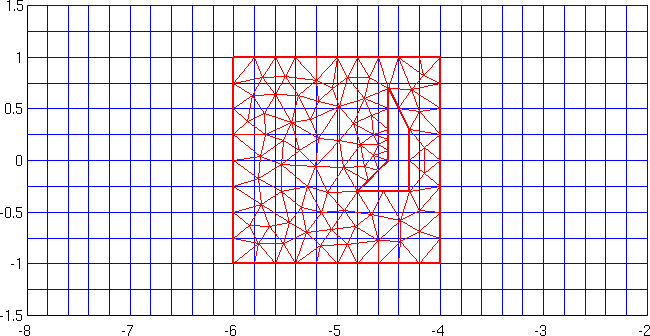
\includegraphics{WavePic/MultiFD_FE_atp5/MultGrid.png}}\par
\end{minipage}
\begin{minipage}{3.3cm}
\centering
\resizebox{3.3cm}{!}{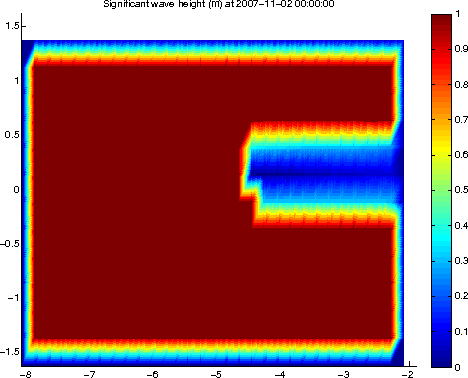
\includegraphics{WavePic/MultiFD_FE_atp5/FD_Hwave_ww0009_20071102_000000.png}}\par
\end{minipage}
\begin{minipage}{3.3cm}
\centering
\resizebox{3.3cm}{!}{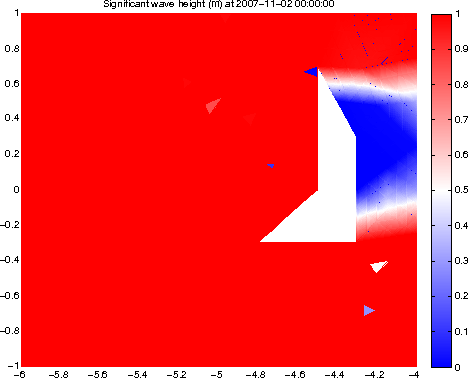
\includegraphics{WavePic/MultiFD_FE_atp5/FE_Hwave_ww0009_20071102_000000.png}}\par
\end{minipage}

\end{center}
Work done with F. Ardhuin (IFREMER), E. Rogers (NRL) and A. Roland (TU Darmstadt)
}


\frame{
  \frametitle{Wave setup}

\begin{itemize}
\item We are considering monochromatic waves of frequency $1.5$ s arriving on a beach and sholaing. We assume $H_s \leq 0.81 d$ as breaking condition.
\end{itemize}

\begin{center}
\begin{minipage}[b]{3.9cm}
\centering
\resizebox{3.9cm}{!}{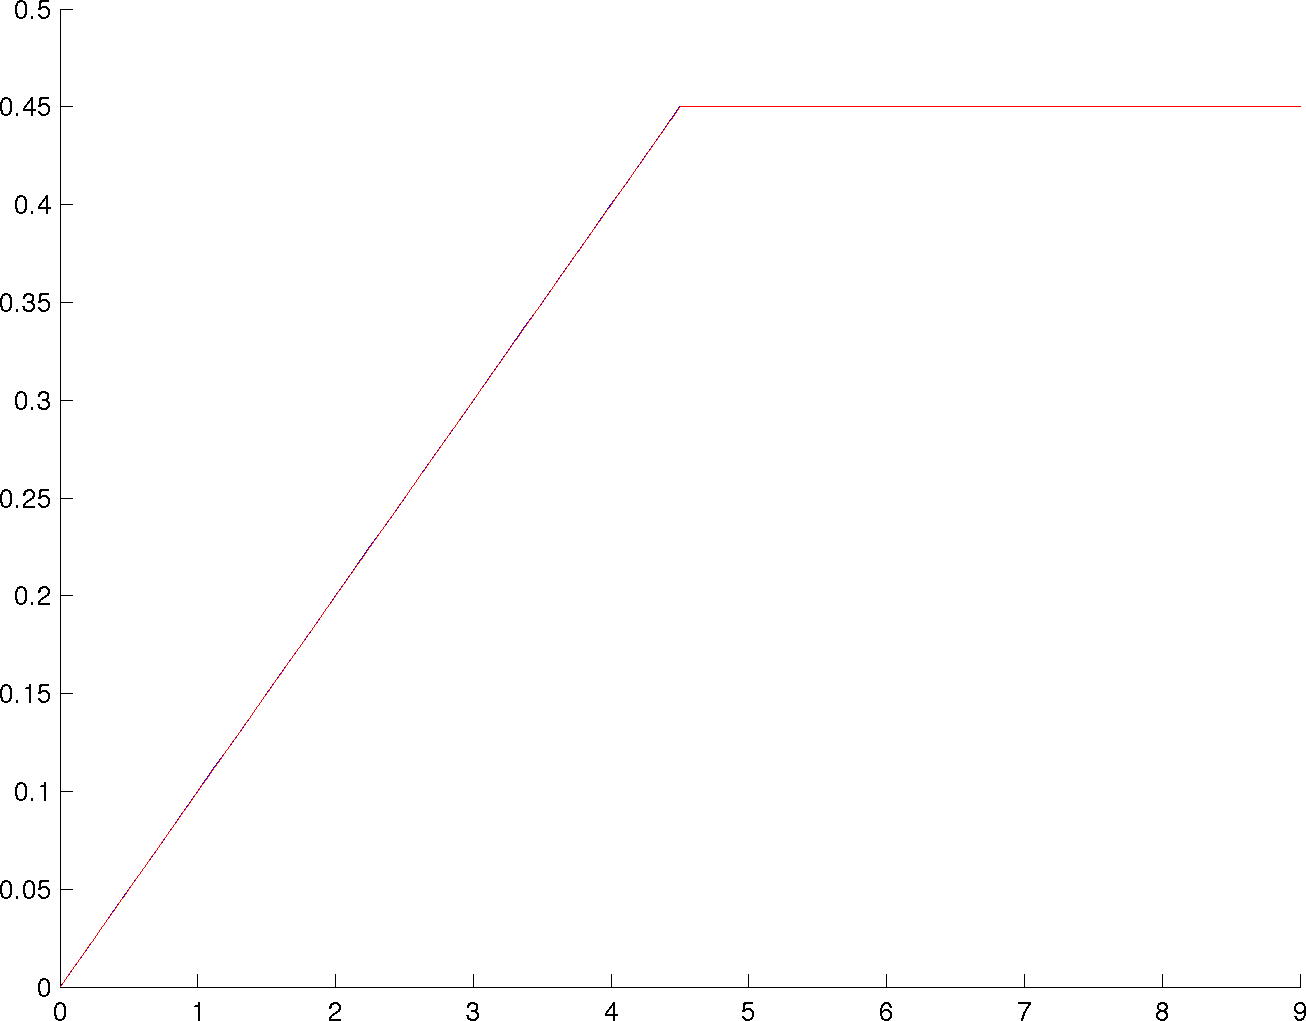
\includegraphics{ImplPic/Setup/LINE_dpt_0004.png}}\par
Depth
\end{minipage}
\begin{minipage}[b]{3.3cm}
\centering
\resizebox{3.3cm}{!}{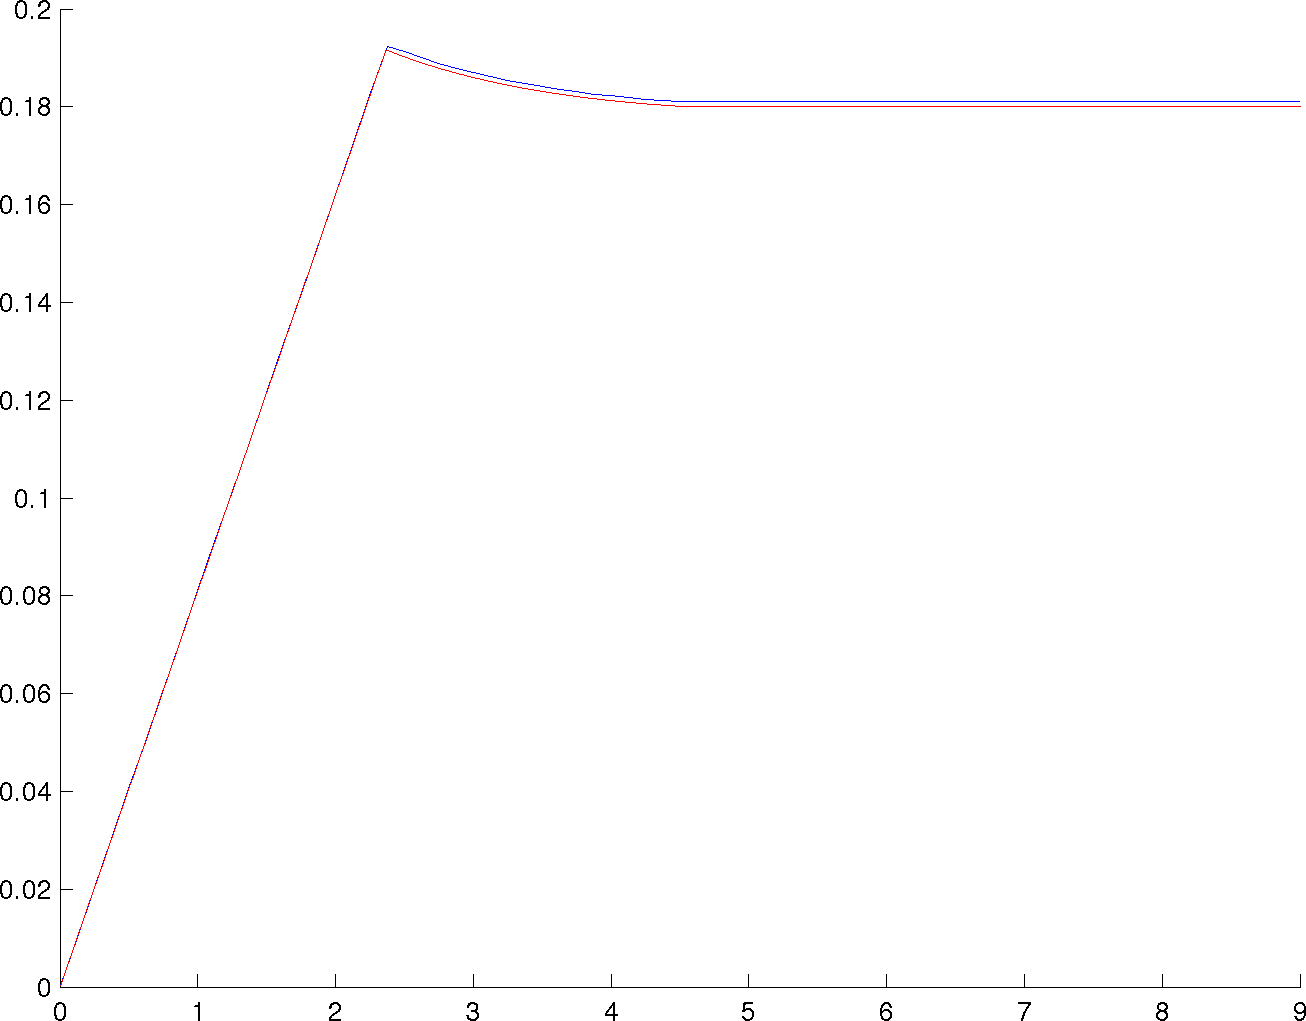
\includegraphics{ImplPic/Setup/LINE_HS_0004.png}}\par
$H_s$
\end{minipage}
\begin{minipage}[b]{3.3cm}
\centering
\resizebox{3.3cm}{!}{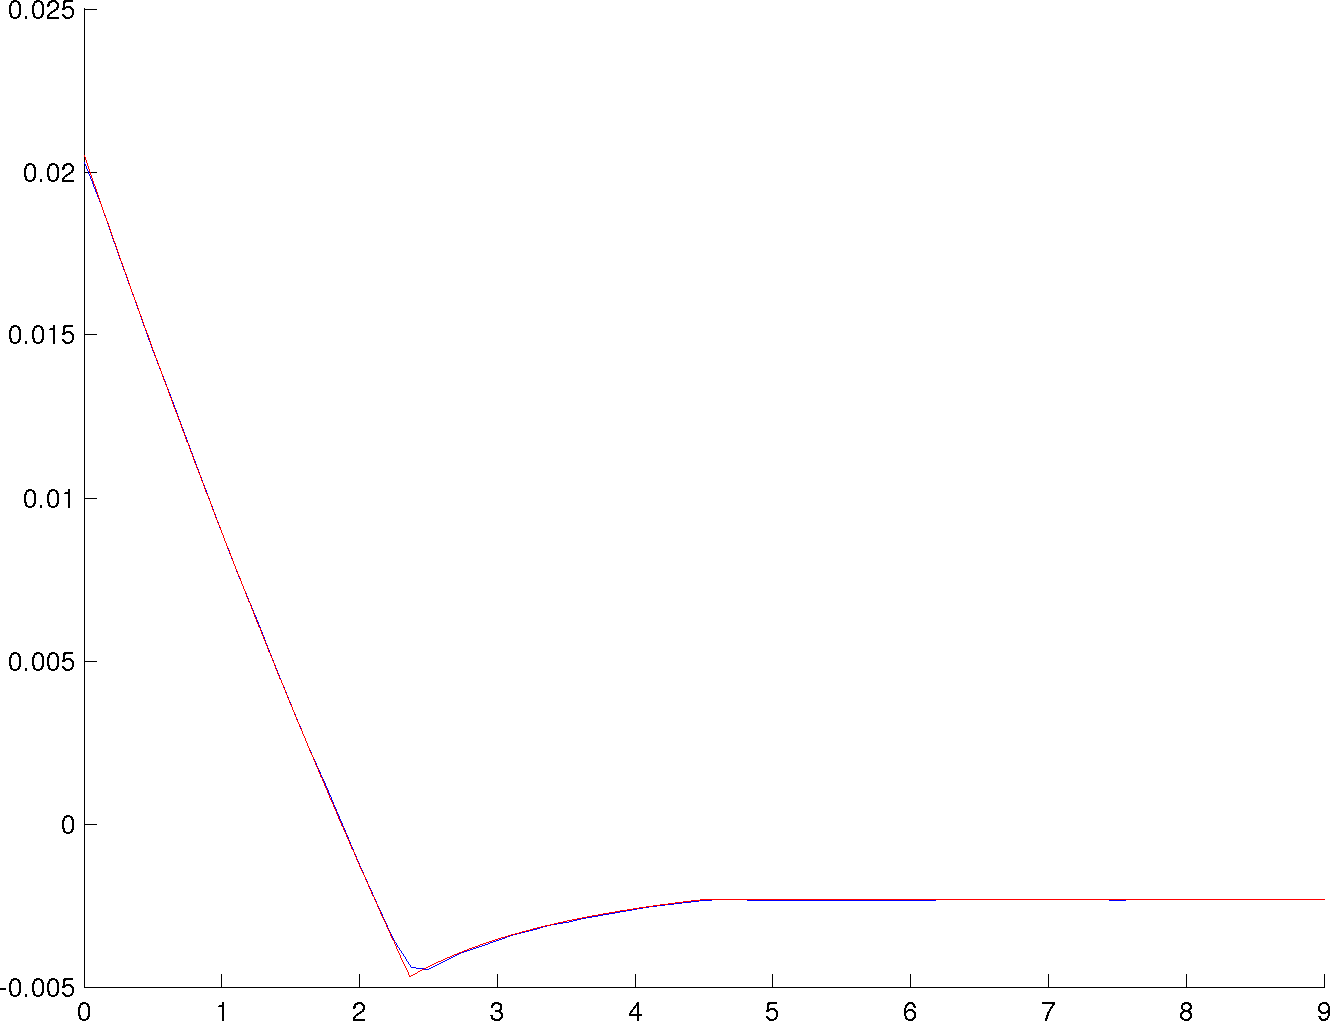
\includegraphics{ImplPic/Setup/LINE_stp_0004.png}}\par
Zeta setup
\end{minipage}

\end{center}

\begin{itemize}
\item The solver used a very simple preconditioner. But the parallelization is very good and the system is very easy to solve.
\item The normalization condition chosen is that the mean of the correction to zeta is $0$.
\end{itemize}

}





\frame{
  \frametitle{High resolution example}
\begin{itemize}
\item The advantage of implicit schemes is the possibility of working with very high resolution grids.
\end{itemize}
\begin{center}
\begin{minipage}[b]{3.9cm}
\centering
\resizebox{3.9cm}{!}{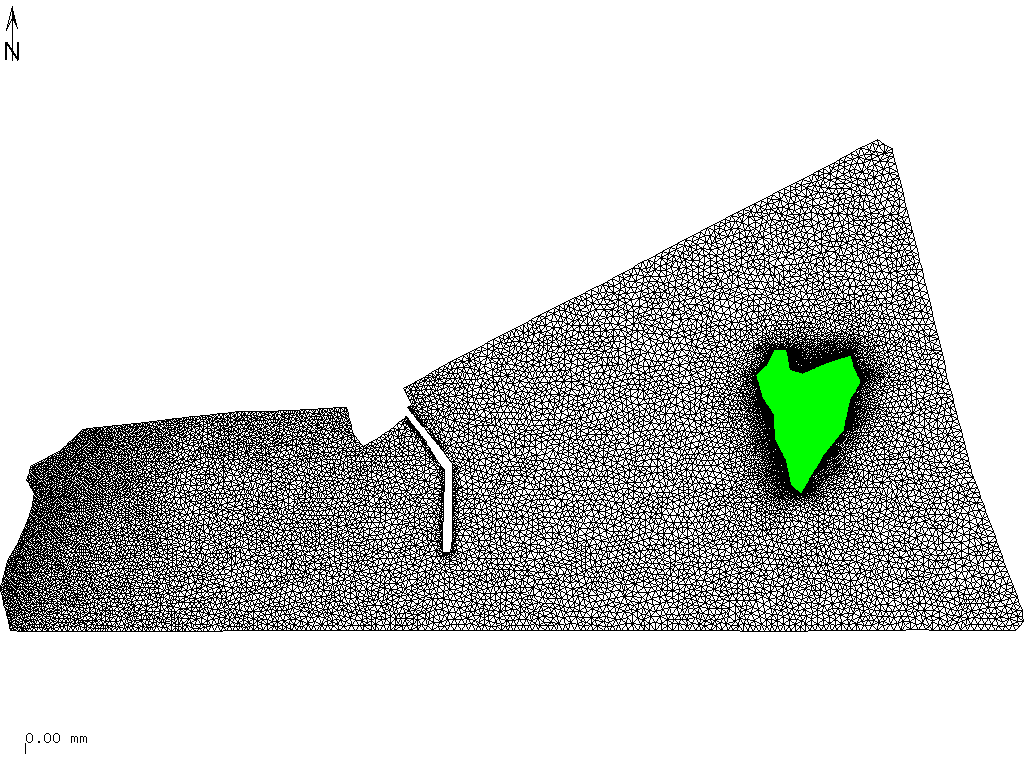
\includegraphics{ImplPic/mesh.png}}\par
The mesh
\end{minipage}
\begin{minipage}[b]{3.3cm}
\centering
\resizebox{3.3cm}{!}{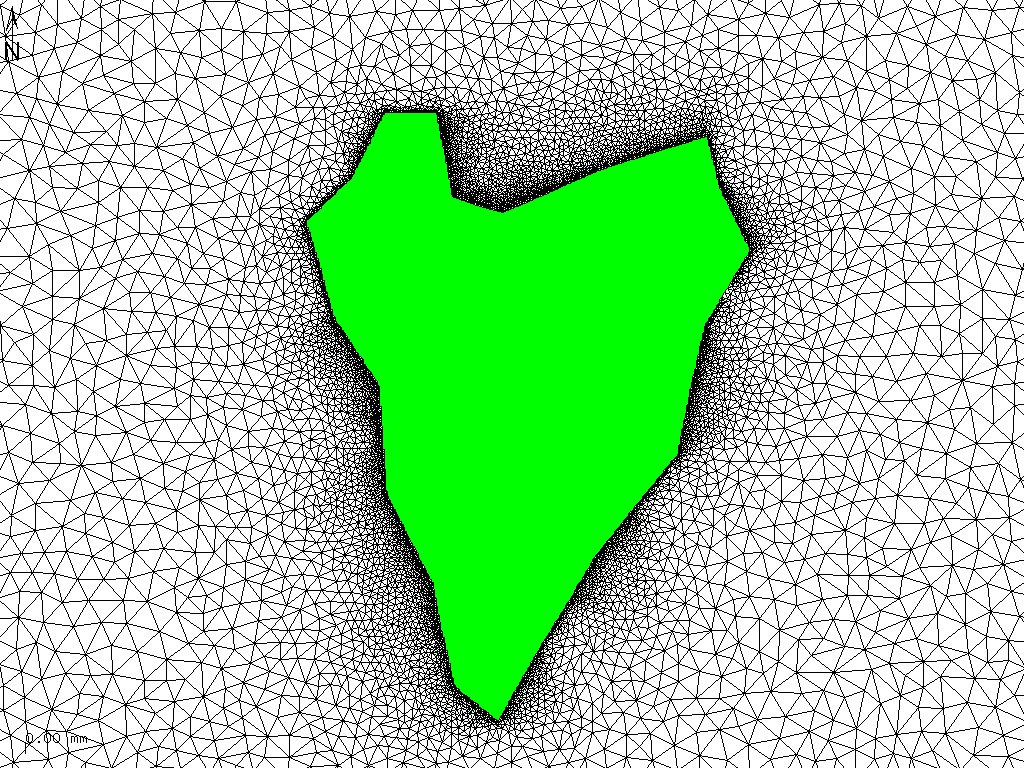
\includegraphics{ImplPic/mesh_detail.png}}\par
Detail of the mesh
\end{minipage}
\begin{minipage}[b]{3.3cm}
\centering
\resizebox{3.3cm}{!}{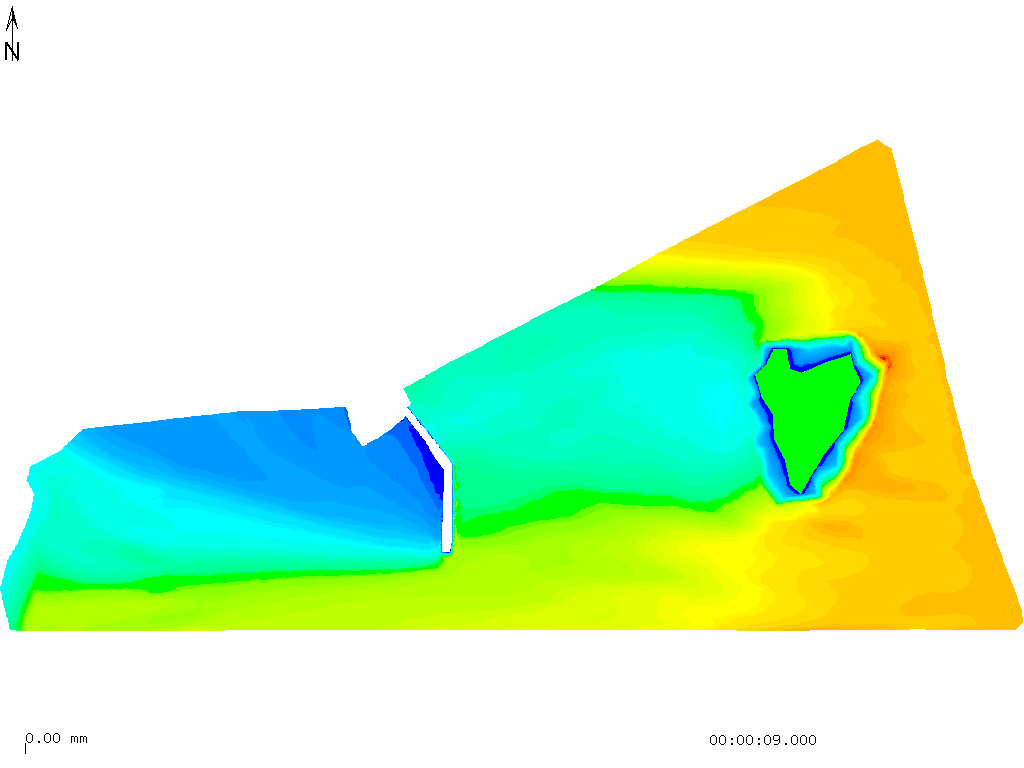
\includegraphics{ImplPic/result.png}}\par
Significant wave height
\end{minipage}
\end{center}
\begin{itemize}
\item For the above 18000 nodes grid, the implicit scheme takes 1 min to solve it while the explicit scheme could not in 30 min.

\end{itemize}
}



\end{document}
